% ============================================================
% TRABAJO FIN DE GRADO / MÁSTER - UNIVERSIDAD DE ZARAGOZA
% ============================================================
% Documento principal (main.tex)
% Compilar con: latexmk -pdf main.tex

\documentclass[a4paper,11pt]{report}

% === PAQUETES BÁSICOS ===
\usepackage[utf8]{inputenc}
\usepackage[T1]{fontenc}
\usepackage[spanish,english]{babel}
\usepackage{csquotes}

% === TIPOGRAFÍA ===
\usepackage{carlito}
\usepackage{anyfontsize}
\renewcommand{\familydefault}{\sfdefault} % Fuente sans-serif oficial UZ (Calibri/Carlito)
\usepackage{setspace}
\onehalfspacing % Establece el interlineado en 1.5 para el documento

% === GEOMETRÍA Y MÁRGENES ===
\usepackage{geometry}
\geometry{
  a4paper,
  left=2.5cm,
  right=2.5cm,
  top=3cm,
  bottom=3cm,
  headheight=14pt
}

% === GRÁFICOS Y COLOR ===
\usepackage{graphicx}
\usepackage[dvipsnames]{xcolor}
\usepackage{subcaption}

% Color corporativo UZ
\definecolor{tfgblue}{RGB}{51,102,153}

% === TABLAS ===
\usepackage{booktabs}
\usepackage{multirow}
\usepackage{array}

% === MATEMÁTICAS ===
\usepackage{amsmath}
\usepackage{amssymb}
\usepackage{amsthm}

% === CÓDIGO FUENTE (LISTINGS) ===
\usepackage{listings}
\lstset{
  basicstyle=\ttfamily\small,
  keywordstyle=\color{blue}\bfseries,
  commentstyle=\color{gray}\itshape,
  stringstyle=\color{red},
  numbers=left,
  numberstyle=\tiny\color{gray},
  stepnumber=1,
  numbersep=8pt,
  backgroundcolor=\color{gray!10},
  frame=single,
  rulecolor=\color{black!30},
  breaklines=true,
  captionpos=b,
  tabsize=2,
  showstringspaces=false
}

% === ALGORITMOS ===
\usepackage[ruled,vlined,linesnumbered,spanish]{algorithm2e}
\SetAlgorithmName{Algoritmo}{algoritmo}{Índice de algoritmos}

% === FORMATO DE CAPÍTULOS Y SECCIONES ===
\usepackage{titlesec}
\titleformat{\chapter}[display]
  {\normalfont\huge\bfseries}{\chaptertitlename\ \thechapter}{20pt}{\Huge}
\titlespacing*{\chapter}{0pt}{-20pt}{40pt}

% === BIBLIOGRAFÍA (IEEE con Biber) ===
\usepackage{csquotes}
\usepackage[
  style=ieee,
  citestyle=numeric-comp,
  sorting=none,
  backend=biber
]{biblatex}
\addbibresource{referencias.bib}

% Configuración para mejor manejo de URLs en la bibliografía
\setcounter{biburlnumpenalty}{9000}
\setcounter{biburlucpenalty}{9000}
\setcounter{biburllcpenalty}{9000}

% === HIPERVÍNCULOS ===
\usepackage[pdfencoding=auto]{hyperref}
\hypersetup{
  colorlinks=true,
  linkcolor=blue!50!black,
  citecolor=green!50!black,
  urlcolor=blue!70!black,
  pdftitle={Título del Trabajo Fin de Grado},
  pdfauthor={Nombre y apellidos del autor},
  pdfsubject={Trabajo Fin de Grado/Máster},
  pdfkeywords={palabra clave 1, palabra clave 2, palabra clave 3},
  bookmarksnumbered=true,
  bookmarksopen=true,
  bookmarksopenlevel=1
}

% === REFERENCIAS CRUZADAS INTELIGENTES ===
\usepackage[spanish,capitalize]{cleveref}
\crefname{figure}{figura}{figuras}
\Crefname{figure}{Figura}{Figuras}
\crefname{table}{tabla}{tablas}
\Crefname{table}{Tabla}{Tablas}
\crefname{equation}{ecuación}{ecuaciones}
\Crefname{equation}{Ecuación}{Ecuaciones}
\crefname{chapter}{capítulo}{capítulos}
\Crefname{chapter}{Capítulo}{Capítulos}
\crefname{section}{sección}{secciones}
\Crefname{section}{Sección}{Secciones}
\crefname{listing}{listado}{listados}
\Crefname{listing}{Listado}{Listados}
\crefname{algorithm}{algoritmo}{algoritmos}
\Crefname{algorithm}{Algoritmo}{Algoritmos}

% === ENCABEZADOS Y PIES DE PÁGINA ===
\usepackage{fancyhdr}
\pagestyle{fancy}
\fancyhf{}
\fancyhead[LE,RO]{\thepage}
\fancyhead[RE]{\leftmark}
\fancyhead[LO]{\rightmark}
\renewcommand{\headrulewidth}{0.4pt}
\renewcommand{\footrulewidth}{0pt}

\fancypagestyle{plain}{
  \fancyhf{}
  \fancyfoot[C]{\thepage}
  \renewcommand{\headrulewidth}{0pt}
  \renewcommand{\footrulewidth}{0pt}
}

% === ANEXOS ===
\usepackage[toc,page]{appendix}
\renewcommand{\appendixtocname}{Anexos}
\renewcommand{\appendixpagename}{Anexos}

% === GLOSARIOS Y ACRÓNIMOS ===
\usepackage[acronym,toc,numberedsection=autolabel]{glossaries}
\makeglossaries

% Definición de ejemplos de acrónimos (edítalos o bórralos)
\newacronym{tfg}{TFG}{Trabajo Fin de Grado}
\newacronym{tfm}{TFM}{Trabajo Fin de Máster}
\newacronym{unizar}{UNIZAR}{Universidad de Zaragoza}

% Definición de términos del glosario
\newglossaryentry{latex}{
  name=LaTeX,
  description={Sistema de composición de textos orientado a la creación de documentos científicos y técnicos de alta calidad tipográfica}
}

% === COMANDOS PERSONALIZADOS ===
\usepackage{xspace}
\newcommand{\ie}{i.e.\xspace}
\newcommand{\eg}{e.g.\xspace}
\newcommand{\etal}{et al.\xspace}

% ============================================================
% INICIO DEL DOCUMENTO
% ============================================================
\begin{document}

% 1. Portada oficial integrada
% ============================================================
% PORTADA OFICIAL (UNIVERSIDAD DE ZARAGOZA)
% ============================================================
% Modifica los textos de esta portada según tus datos

\begin{titlepage}
\thispagestyle{empty}
\centering

% Geometría específica para la portada según directrices
\newgeometry{top=3.24cm, left=2.81cm, right=2.81cm, bottom=2cm}

% Logo de la Universidad

\includegraphics[height=2.4cm]{img/logo_uz.png}\\[1.41cm]

% Caja superior con el tipo de trabajo (e.g., Trabajo Fin de Grado / Trabajo Fin de Máster)
\setlength{\fboxrule}{0.96pt}
\setlength{\fboxsep}{4pt}
\fcolorbox{tfgblue}{white}{%
  \parbox{423.94pt}{\centering\fontsize{28.18}{34}\selectfont
    \vspace{6pt}Trabajo Fin de Grado\vspace{0pt} % Cambiar por Trabajo Fin de Máster si procede
  }%
}\\[2cm]

% Título del trabajo
\fontsize{19.99}{24}\selectfont
Predicción de fibrilación auricular paroxística a partir del electrocardiograma en ritmo sinusal mediante el análisis con redes neuronales profundas \\[0.86cm] % Título en español
{\itshape Prediction of Paroxysmal Atrial Fibrillation from the Sinus Rhythm Electrocardiogram Using Deep Neural Networks}\\[1.5cm] % Título en inglés

% Autor
\fontsize{12.04}{14.5}\selectfont
Autor\\[0.63cm]
\fontsize{18.07}{22}\selectfont
Diego Bouchet Agudo\\[1.2cm]

% Director/es
\fontsize{12.04}{14.5}\selectfont
Directores\\[0.58cm]
\fontsize{13.97}{17}\selectfont
Juan Pablo artínez Cortés \\ Antonio Miguel Artiaga\\[0.78cm]

% Titulación
\fontsize{12.04}{14.5}\selectfont
Titulación\\[0.49cm]
\fontsize{13.97}{17}\selectfont
Grado en Ingeniería de Tecnologías y Servicios de Telecomunicación\\[0.78cm] % Cambiar por tu grado o máster

% Escuela / Facultad y Año
\fontsize{12.04}{14.5}\selectfont
Escuela de Ingeniería y Arquitectura (EINA)\\[0.4cm] % Cambiar por tu centro
\number\year % Genera automáticamente el año actual

\vfill

% Restaurar márgenes normales para el resto de páginas del documento
\restoregeometry
\end{titlepage}


% 2. Páginas preliminares (Numeración romana)
\pagenumbering{Roman}
\setcounter{page}{1}

% Resumen y Abstract
% ============================================================
% RESUMEN / ABSTRACT
% ============================================================

\chapter*{Resumen}
\addcontentsline{toc}{chapter}{Resumen}

\section*{Título del trabajo}
Predicción de fibrilación auricular paroxística a partir del electrocardiograma en ritmo
sinusal mediante el análisis con redes neuronales profundas

\section*{English Title}
{\itshape Prediction of Paroxysmal Atrial Fibrillation from the Sinus Rhythm
Electrocardiogram Using Deep Neural Networks}

\section*{RESUMEN}
\selectlanguage{spanish}

La Fibrilación Auricular Paroxística (PAF) es una de las arritmias más comunes, caracterizada por latidos irregulares en la aurícula.
Debido a su naturaleza intermitente que la caracteriza, su diagnóstico temprano es complejo, es por ello que la predicción de dichos 
episodios a paritr de señales ECG en ritmo sinusal es de especial interés. En este trabajo, se ha abordado este desafío.

Una de las limitaciones que suelen tener trabajos de este tipo es la falta de generalización de los modelos, ya que si son entrenados
en una base de datos específica, de unas características concretas, no suelen generalizar bien a otras bases de datos. 
En este trabajo, se han consolidado cinco bases de datos públicas de PhysioNet para abordar esta limitación. 

Se ha diseñado un preprocesamiento que extrae ventanas inmediatamente anteriores al inicio de un episodio de fibrilación auricular, 
y se extraen nueve variables de variabilidad del ritmo cardíaco (HRV). Se han implementado cuatro arquitecturas distintas de redes neuronales:
ResNet 1D (baseline), SEResNet 1D (con atención de canales), un híbrido CNN-Transformer y Mamba 1D
(\textit{selective state space model}). Para evitar la filtración de datos, se hizo validación cruzada, agrupando estrictamente por sujeto
(5-Fold GroupKFold).

Este trabajo estudia la viabilidad de un sistema generalizable inter-sujeto
para la monitorización de alerta temprana de episodios de Fibrilación Auricular Paroxística.

\vspace{0.8cm}
\noindent\textbf{Palabras clave:} Fibrilación Auricular Paroxística, Predicción Inminente, Procesamiento de ECG, Aprendizaje Profundo, Variabilidad del Ritmo Cardíaco (HRV), Mamba.

\vspace{1cm}

\section*{ABSTRACT}
\selectlanguage{english}

Paroxysmal Atrial Fibrillation (PAF) is one of the most common arrhythmias, characterized by irregular heartbeats in the atrium. Due to its intermittent nature that characterizes it, its early diagnosis is complex; that is why the prediction of such episodes from ECG signals in sinus rhythm is of special interest. In this work, this challenge has been addressed.

One of the limitations that works of this type usually have is the lack of generalization of the models, since if they are trained on a specific database, with concrete characteristics, they do not usually generalize well to other databases. In this work, five public databases from PhysioNet have been consolidated to address this limitation.

A preprocessing has been designed that extracts windows immediately prior to the onset of an atrial fibrillation episode, and nine heart rate variability (HRV) variables are extracted. Four different neural network architectures have been implemented: 1D ResNet (baseline), 1D SEResNet (with channel attention), a hybrid CNN-Transformer, and 1D Mamba (\textit{selective state space model}). To avoid data leakage, cross-validation was performed, grouping strictly by subject (5-Fold GroupKFold).

This work studies the feasibility of an inter-subject generalizable system for early-warning monitoring of Paroxysmal Atrial Fibrillation episodes.

\vspace{0.8cm}
\noindent\textbf{Keywords:} Paroxysmal Atrial Fibrillation, Imminent Prediction, ECG Signal Processing, Deep Learning, Heart Rate Variability (HRV), Mamba.

\selectlanguage{spanish} % Restaurar el idioma principal



% Índices
\clearpage
\tableofcontents

\clearpage
\listoffigures

\clearpage
\listoftables

%\clearpage
%\lstlistoflistings

% Lista de acrónimos / Glosario (Descomentar si se usan)
% \clearpage
% \printglossary[type=\acronymtype,title=Lista de acrónimos]
% \clearpage
% \printglossary[title=Glosario]

% 3. Cuerpo principal del documento (Numeración arábiga)
\clearpage
\pagenumbering{arabic}
\setcounter{page}{1}

% ============================================================
% CAPÍTULO 1: INTRODUCCIÓN
% ============================================================

\chapter{Introducción}
\label{chap:introduccion}

\subsection{Fundamentos de la Electrocardiografía (ECG)}

Un electrocardiograma (ECG) es una representación gráfica de la actividad eleéctrica del corazón en función
del tiempo. Debido a que en cada latido se produce una despolarización y una repolarización de las células,
se generan potenciales eéctricos que pueden ser detectados desde la superficie del cuerpo.

Para capturar esta señal, se colocan electrodos sobre la superficie del cuerpo del paciente, en puntos
específicos, capaces de medir la diferencia de potencial eléctrico generada por este latido. 

La combinación de estos electrodos da lugar a las \textit{derivaciones}. En la práctica,
se suele utilizar el sistema de 12 derivaciones, el cual se divide en:
\begin{itemize}
    \item \textbf{Derivaciones bipolares (I, II, III):} Miden la diferencia de potencial
    entre dos extremidades (siguiendo el triángulo de Einthoven).
    \item \textbf{Derivaciones monopolares aumentadas (aVR, aVL, aVF):} Miden el potencial
    en una extremidad respecto a un punto de referencia central.
    \item \textbf{Derivaciones precordiales (V1 a V6):} Situadas directamente sobre el tórax para
    observar la actividad eléctrica en el plano horizontal del corazón.
\end{itemize}

\begin{figure}[htbp]
  \centering
  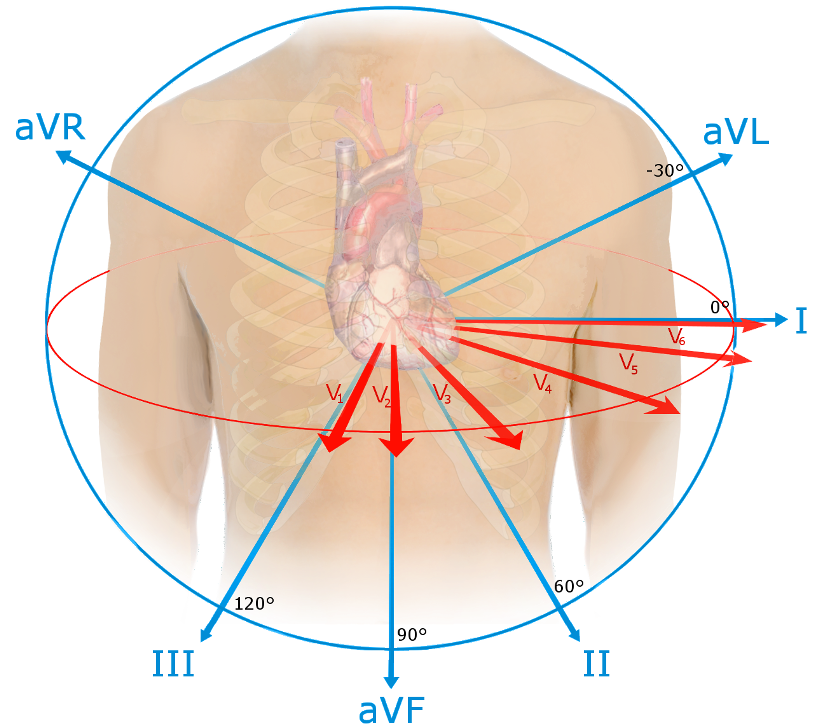
\includegraphics[width=0.5\textwidth]{img/EKG_leads.png}
  \caption{Orientación espacial de las derivaciones ECG. Imagen obtenida de \href{https://en.wikipedia.org/wiki/Electrocardiography}{Wikipedia}.}
  \label{fig:orientacion_derivaciones}
\end{figure}

Cada derivación observa el mismo fenómeno eléctrico, pero desde un ángulo espacial distinto. Esto resulta
clave para la detección de patologías como arritmias o infartos. \cite{wikipedia_electrocardiography_2026}

% ---------- cambiar si hay timepo hacia arriba

La Fibrilación Auricular (FA) es la arritmia cardíaca más común, caracterizada por un comportamiento
auricular caótico (como se ilustra en la Figura~\ref{fig:ejemplo}).
Esta patología provoca una pérdida de la contracción auricular efectiva, lo que incrementa
el riesgo de formación de trombos, accidentes cerebrovasculares (ictus), insuficiencia cardíaca
y deterioro cognitivo a largo plazo \cite{wikipedia_atrial_2026}.

\begin{figure}[htbp]
  \centering
  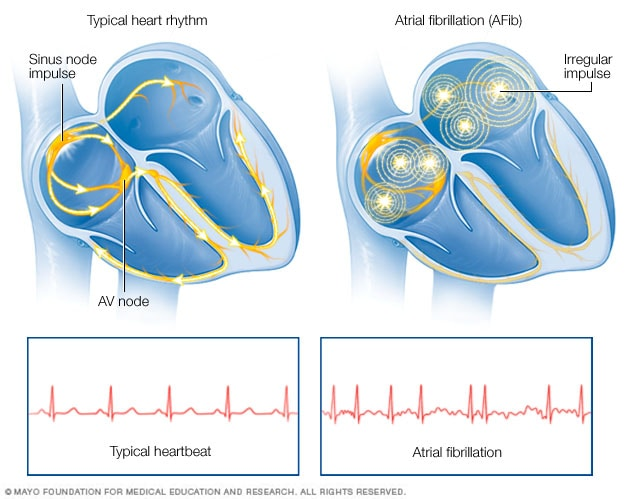
\includegraphics[width=0.7\textwidth]{img/atrial fibrilation.jpg}
  \caption{Ejemplo de ECG en fibrilación auricular. Imagen obtenida de la \href{https://www.mayoclinic.org/diseases-conditions/atrial-fibrillation/symptoms-causes/syc-20350624}{Mayo Clinic}.}
  \label{fig:ejemplo}
\end{figure}

Dentro de sus varaintes, se encuentra la Fibrilación Auricular Paroxística (PAF, por sus siglas en
inglés, \textit{Paroxysmal Atrial Fibrillation}). Ésta se caracteriza por episodios esporádicos de arritmia,
que se inician de manera espontánea y que vuelven al ritmo sinusal en un periodo de unos 7 días, aunque la mayoría lo hacen en menos de 24 horas.

Debido a esta naturaleza intermitente, los ECGs de corta duración no suelen capturarlos. Por ello, la predicción inminente de estos episodios, 
es decir, tener la capacidad de predecir si un paciente sufrirá un episodio en los próximos
minutos a partir de su ritmo sinusal, en holters de larga duración es de especial interés.

Predecir un episodio con una ventana de antelación de hasta 5 minutos permitiría alertar al paciente para que cese
actividades de riesgo, automatizar la administración preventiva de fármacos
antiarrítmicos o preparar dispositivos de estimulación eléctrica cardíaca adaptativa.

Sin embargo, la predicción es una tarea compleja. La fase previa al episodio arrítmico es en ritmo sinusal,
por lo que a simple vista en el ECG no se observan patrones o anomalías morfológicas evidentes.

\section{Contexto del Trabajo}
\label{sec:contexto}

Clasicamente este problema solia abordarse mediante la extracción de características de
variabilidad del ritmo cardíaco (HRV, \textit{Heart Rate Variability}) y por un clasificador lineal. Sin embargo esta
estrategia no suele ser capaz de analizar las distorsiones morfológicas locales de las señales
de ECG (como cambios finos en la onda P o en el intervalo PR) que preceden a la FA.

Las redes neuronales cambian la forma de abordar este problema, permitiendo extraer información
directamente de la señal ECG sin procesar. No obstante hay que tener en cuenta algunas limitaciones
como:

\begin{enumerate}
  \item \textbf{Sesgo de Base de Datos:} Se entrenan utilizando una única base
  de datos. Esto genera modelos altamente sobreajustados a las condiciones de ruido y
  hardware de esa base de datos concreta, que fracasan al ser validados en registros
  independientes.
  \item \textbf{Data Leakage y validaciones débiles:} Con frecuencia se comparten
  ventanas del mismo paciente entre los conjuntos de entrenamiento y test,
  reportando precisiones artificialmente altas.
\end{enumerate}

Este trabajo se enfoca en resolver estas limitaciones utilizando un dataset
procedente de distintas bases de datos, evaluando los modelos mediante una validación cruzada inter-sujeto.


\section{Objetivos del Proyecto}
\label{sec:objetivos}

El objetivo de este proyecto es
\textbf{diseñar, implementar y evaluar un sistema capaz de
predecir de forma inminente (en una ventana de 5 minutos antes del inicio) episodios de
Fibrilación Auricular Paroxística (PAF) a partir de segmentos de 1 minuto de señal ECG en
ritmo sinusal}.

Para alcanzar este fin, se definen los siguientes objetivos:
\begin{itemize}
  \item \textbf{Objetivo 1:} 
  Integrar cinco bases de datos heterogéneas de PhysioNet:
  \textit{afpdb}, \textit{cpsc2021}, \textit{ltafdb}, \textit{shdb-af} y \textit{afdb}.
  \item \textbf{Objetivo 2:} 
  Desarrollar un pipeline de preprocesamiento que permita la
  extracción de ventanas variables de ritmo sinusal Pre-PAF y de características
  temporales y frecuenciales de HRV.
  \item \textbf{Objetivo 3:} 
  Entrenar distintas arquitecturas de redes neuronales como: ResNet 1D (modelo base residual),
  SEResNet 1D (con atención por canal Squeeze-and-Excitation),
  un modelo CNN-Transformer (\textit{multi-head self attention})
  y Mamba 1D (basado en \textit{state space models}).
  \item \textbf{Objetivo 4:} 
  Integrar la información de HRV mediante una cabeza clasificatoria
  (Multi-Layer Perceptron) que potencie la toma de decisiones de
  las redes.
  \item \textbf{Objetivo 5:} 
  Evaluar rigurosamente los modelos bajo un diseño GroupKFold para mitigar
  la filtración de datos.
\end{itemize}



% ============================================================
% CAPÍTULO 2: DATOS
% ============================================================

\chapter{Datos}
\label{chap:datos}

La adquisición de datos de calidad es fundamental para el desarrollo de modelos capaces
de predecir con generalidad y fiabilidad. Por ello se han incorporado varias bases de datos
obtenidas de fuentes públicas, en concreto, de los repositorios de PhysioNet.
Estas bases de datos contienen registros de electrocardiogramas (ECG) con anotaciones
sobre episodios de fibrilación auricular paroxística (PAF).

\section{Bases de datos utilizadas}
\label{sec:bases_datos}

Para el desarrollo de este proyecto se han empleado 5 bases de datos detalladas a continuación:

\subsection{PAF Prediction Challenge Database (afpdb)}
\label{subsec:afpdb}
Esta base de datos~\cite{moody_paf_2001} fue diseñada para el PhysioNet Challenge de predicción de
Fibrilación Auricular Paroxística. Contiene registros de ECG de dos canales con
una duración de 30 minutos y una frecuencia de muestreo de 128~Hz. El conjunto de
aprendizaje consta de 50 parejas de registros (100 registros en total) procedentes
de 48 sujetos:
\begin{itemize}
  \item \textbf{Registros tipo 'n':} 50 registros procedentes de sujetos sanos o sin antecedentes de Fibrilación Auricular.
  \item \textbf{Registros tipo 'p':} 50 registros obtenidos inmediatamente antes de un episodio de Fibrilación Auricular (Pre-PAF).
\end{itemize}
Adicionalmente, existe un conjunto de test con otros 100 registros procedentes de 50 sujetos, que utilizaremos para compararnos
con otros trabajos publicados.

\subsection{China Physiological Signal Challenge 2021 (cpsc2021)}
\label{subsec:cpsc2021}
Esta base de datos~\cite{PhysioNet-cpsc2021-1.0.0} contiene 1425 registros de 105 sujetos,
dos canales, muestreadas a 200~Hz. Contiene anotaciones
de ritmo, en concreto, de inicio y fin de episodios de Fibrilación Auricular.

\subsection{Long-Term Atrial Fibrillation Database (ltafdb)}
\label{subsec:ltafdb}
Esta base de datos~\cite{petrutiu_long-term_2003} contiene registros de ECG ambulatorio de
larga duración (aproximadamente 24 horas por registro), grabados a una frecuencia de muestreo
de 128~Hz. Consta de 84 registros de 84 sujetos con fibrilación auricular
paroxística o sostenida.

\subsection{Smart Health Devices - Atrial Fibrillation Database (shdb-af)}
\label{subsec:shdb}
Esta base de datos~\cite{PhysioNet-shdb-af-1.0.1} proporciona señales de ECG de dos
canales registradas mediante dispositivos wearables en condiciones cotidianas.
Consta de 128 registros
de larga duración (24 horas) procedentes de 122 sujetos con PAF,
muestreados originalmente a 125~Hz y resampleados a 200~Hz.
Nos proporciona la asignación entre señal y sujeto para prevenir filtraciones (leakage)

\subsection{MIT-BIH Atrial Fibrillation Database (afdb)}
\label{subsec:afdb}
Esta base de datos~\cite{moody_mit-bih_1992} consta de 25 registros de ECG de dos
canales con una duración de 10 horas cada uno, grabados a 250~Hz.
Cabe destacar que de 25, 23 de estos registros contienen señales de
ECG utilizables, ya que los otros 2 constan únicamente de anotaciones.

\section{Características comparativas de los conjuntos de datos}
\label{sec:caracteristicas_datos}

A continuación se presenta una tabla~\ref{tab:resumen_datos} que resume las características de las 5 bases de datos utilizadas
en este proyecto, incluyendo el número de pacientes, el número de registros, el número
de canales y la frecuencia de muestreo de cada base de datos.

\begin{table}[htbp]
  \centering
  \caption{Resumen comparativo de las 5 bases de datos de estudio}
  \label{tab:resumen_datos}
  \begin{tabular}{lcccc}
    \toprule
    \textbf{Base de datos} & \textbf{Nº Pacientes} & \textbf{Nº Registros} & \textbf{Canales} & \textbf{Frec. Muestreo} \\
    \midrule
    \texttt{afpdb~\cite{moody_paf_2001}} & 48 (98) & 100 (300) & 2 & 128 Hz \\
    \texttt{cpsc2021~\cite{PhysioNet-cpsc2021-1.0.0}} & 105 & 1425 & 2 & 200 Hz \\
    \texttt{ltafdb~\cite{petrutiu_long-term_2003}} & 84 & 84 & 2 & 128 Hz \\
    \texttt{shdb-af~\cite{PhysioNet-shdb-af-1.0.1}} & 122 & 128 & 2 & 200 Hz \\
    \texttt{afdb~\cite{moody_mit-bih_1992}} & 25 & 25 (23) & 2 & 250 Hz \\
    \bottomrule
  \end{tabular}
  \vskip 5pt
  \small
  \textit{Nota:} Para \texttt{afpdb}, entre paréntesis se indica el total incluyendo el conjunto de test. Para \texttt{afdb}, entre paréntesis se indica el número de registros que contienen señales utilizables.
\end{table}

% ============================================================
% CAPÍTULO 3: METODOLOGÍA
% ============================================================

\chapter{Metodología}
\label{chap:metodologia}

A continuación se detallan los métodos que se han seguido para la descarga, preprocesamiento
de las señales, extracción de características de variabilidad de ritmo cardíaco  (HRV),
y las arquitecturas de las redes neuronales utilizadas para la predicción de
Fibrilación Auricular a partir de segmentos de ECG en ritmo sinusal.

\section{Descarga y lectura de bases de datos}
\label{sec:descarga}

La descarga de bases de datos se ha realizado desde el Clúster del Instituto de Investigación en
Ingeniería de Aragón (I3A)\footnote{\url{https://i3a.unizar.es/es}}, en concreto, en el grupo de investigación BSICoS\footnote{\url{https://bsicos.i3a.es/}},
utilizando el gestor de descargas \texttt{wget}.

Para la lectura, se ha utilizado la librería \texttt{wfdb} de Python,
que permite leer los registros ECG y extraer las anotaciones correspondientes.
Puesto que el trabajo se centra en la predicción inminente, se han extraido ventanas
inmediatamente anteriores a los episodios de fibrilación auricular (Pre-PAF), en concreto,
de un máximo de 5 minutos anteriores al episodio, además de segmentos de control de ritmo sinusal estable.

Cada registro se ha cargado en memoria como un array de \texttt{NumPy} para su posterior procesamiento.


\section{Preprocesamiento}
\label{sec:preprocesamiento}

El preprocesamiento es esencial por varias razones: las bases de datos utilizadas no
presentan la misma frecuencia de muestreo, ni están medidas con el mismo equipo, por tanto
hay que implementar un pipeline que unifique las características para que los modelos puedan generalizar correctamente.
El pipeline de preprocesamiento consta de tres pasos principales:

\begin{enumerate}
  \item \textbf{Armonización de Canales y Frecuencia de Muestreo:}
  Se unifican todas las señales a exactamente dos canales y una frecuencia de
  muestreo de $128$~Hz. Si un registro tiene menos de dos canales, se realiza un relleno
  (padding) con ceros, si tiene más, se seleccionan únicamente las dos primeras
  derivaciones. En nuestro caso todas las bases de datos contienen 2 canales, pero se comprueba
  por generalidad, para tener la posibilidad de añadir posteriormente bases de datos adicionales.
  El remuestreo se ejecuta mediante interpolación trigonométrica.
  \item \textbf{Atenuación del Ruido e Interferencia:}
  La tarea de la eliminación del ruido se delega a las primeras capas convolucionales de los moedlos,
  que aprenderán los filtros necesarios para su correcta eliminación, optimizados para la tarea.
  \item \textbf{Normalización Z-score Local:}
  Para evitar sesgos debido a las variaciones inter-sujeto o inter-dispositivo en la
  amplitud absoluta de las señales, cada segmento se normaliza de forma independiente
  por canal en el dataloader aplicando:
  \begin{equation}
  x_{\text{norm}} = \frac{x - \mu}{\sigma + 10^{-8}}
  \end{equation}
  donde $\mu$ y $\sigma$ representan la media y desviación estándar de la amplitud
  de cada ventana.
\end{enumerate}


\section{Extracción de Ventanas y Prevención de Data Leakage}
\label{sec:extraccion_ventanas}

Los dos tipos de
segmentos requeridos para la clasificación binaria son:

\begin{itemize}
  \item \textbf{Clase 1 (Pre-PAF):}
  Esta clase representa el estado inmediatamente anterior a un episodio de fibrilación auricular. Se ha optado por extraer
  ventanas de longitud variable, de entre $60$ ($1$ minuto) y $300$ ($5$ minutos) segundos, que parten desde el inicio del episodio
  y retroceden en el timepo hasta 5 minutos, o hasta encontrarse con el inicio de otro episodio. De esta manera, se garantiza
  que el segmento contenga solamente ritmo sinusal.

  \item \textbf{Clase 0 (Normal/Control):}
  Se extraen segmentos estables de ritmo sinusal
  de $5$ minutos de duración, que se encuentren alejados al menos $30$ minutos
  ($1800$ segundos) de cualquier episodio
  (tanto antes como después), para evitar zonas de transición.

  Esto es importante, ya que estamos extrayendo ventanas de clase normal de pacientes 
  tanto con PAF como sanos.

  Esta estrategia es fundamental.
  Si la Clase 0 se compusiera solo de individuos sanos, los modelos aprenderían a identificar
  diferencias morfológicas asociadas a la cardiopatía estructural del paciente, en lugar de identificar
  los cambios transitorios que desencadenan el episodio.

\end{itemize}

Para evitar la filtración de datos (\textit{data leakage}), los segmentos se agrupan estrictamente por sujeto.
Esto garantiza que en validación y test no haya pacientes que ya hayan aparecido en
el entrenamiento, ya que el modelo podría aprender a reconocer la morfología de un paciente concreto en lugar de
aprender a generalizar la predicción de la fibrilación auricular.


\section{Aumento de Datos (Data Augmentation)}
\label{sec:aumentacion}

Debido a que los modelos escalan mejor con grandes cantidades de datos, se ha 
implementado un pipeline de aumento de datos, que aplica modificaciones realistas a las
señales directamente en el dataloader con una probabilidad
del $50\%$ para cada una:
\begin{itemize}
  \item \textbf{Deriva de la Línea de Base (\textit{Baseline Wander}):} Se simula la deriva lenta causada por la respiración del paciente sumando una señal sinusoidal:
  \begin{equation}
  x_{\text{aug}}(t) = x(t) + A \cdot \sin(2\pi \cdot f \cdot t)
  \end{equation}
  donde la frecuencia $f$ se muestrea de manera uniforme en $[0.1, 0.5]$~Hz y la amplitud $A$ en $[0.05, 0.2]$.
  \item \textbf{Ruido Gaussiano Aditivo:} Se simula el ruido instrumental sumando ruido blanco gaussiano con una desviación estándar variable $\sigma_{\text{noise}} \sim U(0.01, 0.05)$.
  \item \textbf{Escalado Aleatorio:} Se multiplica el segmento por un factor de escala $s \sim U(0.85, 1.15)$ para simular fluctuaciones en la ganancia del amplificador.
  \item \textbf{Slice Aleatorio de Ventana:} Dado que las redes se entrenan con ventanas
  de $60$ segundos, y contamos con señales de hasta 5 minutos, se extraen 60 segundos aleatorios.
  En validación y test, se toma de forma determinista los últimos $60$ segundos
  (el instante más cercano al inicio de la crisis en la Clase 1).
\end{itemize}

En la figura~\ref{fig:data_augmentation_demo} se ilustra una demostración visual del efecto individual y
combinado de estas técnicas de aumentación de datos aplicadas a un segmento real de electrocardiograma.

\begin{figure}[htbp]
  \centering
  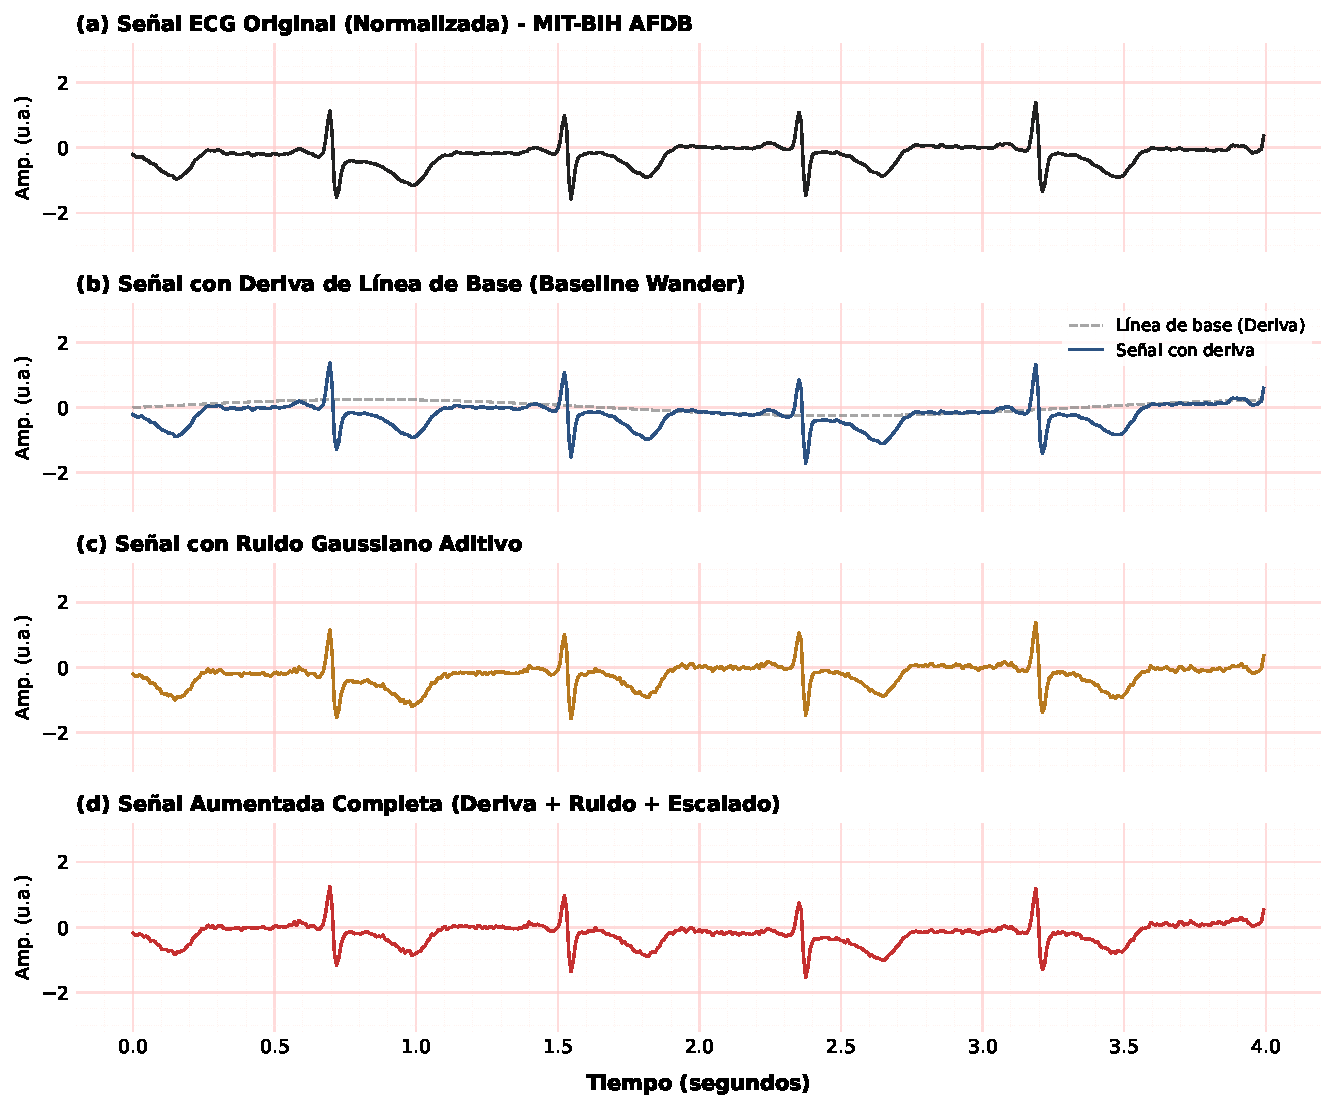
\includegraphics[width=0.9\textwidth]{img/data_augmentation_demo.pdf}
  \caption{Efecto del aumento de datos sobre un segmento de ECG de 4 segundos. Se muestra (a) la señal original
normalizada, (b) la adición de deriva lenta (baseline wander), (c) la adición de ruido de alta frecuencia, y (d) el
resultado combinado de todas las transformaciones.}
  \label{fig:data_augmentation_demo}
\end{figure}

\section{Extracción de Variabilidad del Ritmo Cardíaco (HRV)}
\label{sec:hrv}

Como información complementaria, se calculan nueve variables de variabilidad de ritmo cardíaco (HRV)
a partir de las anotaciones de los picos QRS procedentes de las bases de datos, utilizando las ventanas
de ritmo sinusal de 5 minutos. (Reescalados a $128$~Hz)

\begin{itemize}
      \item \textbf{Métricas Temporales:}
      \begin{itemize}
          \item \textit{Media de intervalos RR} (\texttt{mean\_rr}): Promedio aritmético de los intervalos, expresado en segundos.
          \item \textit{Desviación estándar de intervalos RR} (\texttt{std\_rr}): Medida de la variabilidad global del registro.
          \item \textit{RMSSD} (\texttt{rmssd}): Raíz cuadrada de la media de las diferencias al cuadrado de intervalos sucesivos:
          \begin{equation}
              \text{RMSSD} = \sqrt{\frac{1}{N-1} \sum_{i=1}^{N-1} (RR_{i+1} - RR_i)^2}
          \end{equation}
          \item \textit{pNN50} (\texttt{pnn50}): Porcentaje de intervalos sucesivos que difieren en más
          de $50\text{ ms}$:
          \begin{equation}
              NN50 = \text{Número de intervalos } i \text{ tales que } |RR_{i+1} - RR_i| > 0.05\text{ s}
          \end{equation}
          \begin{equation}
              pNN50 = \frac{NN50}{N - 1} \times 100
          \end{equation}
          donde $N$ representa el número de intervalos $RR$ totales analizados en el segmento.
          \item \textit{Frecuencia cardíaca instantánea} (\texttt{mean\_hr} y \texttt{std\_hr}):
          Obtenida para cada intervalo mediante $\text{HR}_i = 60 / RR_i$
          y calculando su media y desviación estándar.
      \end{itemize}

      \item \textbf{Métricas Frecuenciales:}
      Dado que la serie de intervalos $RR$ es una señal discreta de frecuencia de muestreo no uniforme debido
      a que depende de cada latido, se requiere un preprocesamiento para estimar la Densidad Espectral
      de Potencia (PSD):
      \begin{itemize}
          \item \textit{Interpolación y Remuestreo:} A partir de la serie temporal acumulada de los
          intervalos $RR$, se realiza una interpolación lineal y un remuestreo uniforme a una frecuencia
          fija de $4\text{ Hz}$ para que supere el límite de Nyquist requerido para la
          banda superior de ($0.40\text{ Hz}$). A la señal remuestreada se le elimina su valor
          medio para eliminar la componente de continua ($0\text{ Hz}$) y evitar distorsiones en las
          frecuencias bajas.

          \item \textit{Estimación de la PSD (Método de Welch):}
          Se aplica el método de Welch sobre la serie remuestreada a $4\text{ Hz}$
          utilizando segmentos solapados de $256$ muestras. De esta manera se establece un compromiso entre
          resolución en frecuencia y reducción de la varianza del estimador espectral.
          \item \textit{Energía en baja frecuencia} (\texttt{lf}):
          Potencia integrada en el rango $[0.04, 0.15)\text{ Hz}$.
          \item \textit{Energía en alta frecuencia} (\texttt{hf}):
          Potencia integrada en el rango $[0.15, 0.40]\text{ Hz}$.
          \item \textit{Relación de balance autonómico} (\texttt{lf\_hf\_ratio}):
          \begin{equation}
            \frac{\text{LF}}{\text{HF} + 10^{-8}}
          \end{equation}.
      \end{itemize}
      El límite inferior de $60$ segundos para la longitud de la ventana se ha establecido para garantizar la estabilidad
      de las métricas de HRV frecuenciales, en concreto, de la banda de baja frecuencia (LF),
      que requiere un mínimo de $1/0.04 = 25$ ciclos para una estimación confiable. Una ventana de $60$ segundos asegura al
      menos $2.4$ ciclos completos de dicha oscilación.

  \end{itemize}



\section{Arquitecturas de Aprendizaje Profundo}
\label{sec:arquitecturas}

Se proponen cuatro arquitecturas para procesar la señal de entrada $\mathbf{X} \in \mathbb{R}^{2 \times L}$ (donde $L = 7680$ muestras para una ventana de $60$ segundos a $128$~Hz):

\subsection{ResNet 1D (Baseline)}
Basada en bloques convolucionales 1D residuales\cite{rajpurkar2017cardiologistlevelarrhythmiadetectionconvolutional}. Cada bloque residual consta de capas
convolucionales seguidas de (\textit{Batch Normalization}),
activación ReLU y una \textit{skip connection}\cite{he2015deepresiduallearningimage} que suma la entrada
original a la salida del bloque, lo que facilita el paso de gradiente en arquitecturas profundas
(véase el diagrama de la figura~\ref{fig:resnet} del anexo~\ref{appendix:arquitecturas}).



\subsection{SEResNet 1D (Atención de Canales)}
Añade bloques \textit{Squeeze-and-Excitation} (SE) tras cada bloque residual.
El bloque SE comprime la información espacial del canal mediante un
\textit{Global Average Pooling} y, a través de una pequeña red \textit{fully connected}
con cuello de botella, calcula un peso de excitación para cada canal.
Esto permite a la red ponderar la importancia relativa de cada una de las dos
derivaciones del ECG de forma dinámica. \cite{senet1d}
(Vease el anexo~\ref{appendix:arquitecturas}).

\subsection{CNN-Transformer Híbrido}
Combina las fortalezas de las redes convolucionales y los mecanismos de atención.
Las capas convolucionales iniciales extraen rasgos morfológicos locales y reducen la
dimensión temporal de la secuencia. Posteriormente, el Transformer procesa
la secuencia resultante. Utilizando mecanismos de \textit{Multi-Head Self-Attention},
el Transformer captura dependencias temporales a lo largo de todo el segmento de ECG
(Vease el anexo~\ref{appendix:arquitecturas}).\cite{vaswani2023attentionneed}

\subsection{Mamba 1D (Modelo de Espacio de Estados)}
Como alternativa al Transformer, se implementa una arquitectura
basada en \textit{State space models} (SSM) de selección variable (Mamba).
Mamba parametriza un sistema lineal invariante en el tiempo que procesa la señal a través
de una recurrencia lineal selectiva y dependiente de los datos. Esto permite capturar
dependencias de largo alcance con una complejidad computacional que escala linealmente
$O(L)$ en lugar de cuadrática $O(L^2)$ como ocurre con en el Transformer
(Vease el anexo~\ref{appendix:arquitecturas}).

\subsection{Integración de Características HRV}
Adicionalmente, se concatenan a la salida de los modelos a la cabeza clasificatoria (MLP)
las 9 variables de HRV. Finalmente, esta representación combinada se introduce en una capa lineal clasificadora
con activación Softmax para emitir la probabilidad de Pre-PAF.

\section{Estrategia de Evaluación y Validación Cruzada}
\label{sec:estrategia_evaluacion}

El diseño experimental se define mediante:
\begin{itemize}
  \item \textbf{Validación Cruzada (5-Fold GroupKFold):}
  El dataset total se divide en 5 \textit{folds} de forma que todos los segmentos de un mismo
  paciente queden en el mismo \textit{fold}. En cada iteración, se entrenan los modelos en
  4 \textit{folds} y se validan en el restante.
  \item \textbf{Evaluación Externa:}
  Para comparar los modelos en igualdad de condiciones con la literatura científica, los modelos se evalúan adicionalmente en el conjunto de prueba independiente de la base de datos \texttt{afpdb} (PAF Prediction Challenge).
  \item \textbf{Métricas de Calidad:} Se evalúa el rendimiento utilizando la sensibilidad (Recall), especificidad, precisión, puntuación F1 macro (F1 Macro), F1 de la clase Pre-PAF (F1 Clase 1) y el área bajo la curva ROC (AUC-ROC).
\end{itemize}

% ============================================================
% CAPÍTULO 4: RESULTADOS
% ============================================================

\chapter{Resultados y Discusión}
\label{chap:resultados}

En este capítulo se presentan los resultados obtenidos por las cuatro
arquitecturas implementadas (ResNet 1D, SEResNet 1D, el modelo
híbrido CNN-Transformer y Mamba 1D). El entrenamiento se ha realizado mediante
una validación cruzada por grupos (5-Fold Group Cross-Validation),
asegurando que los registros de un mismo sujeto
nunca se compartan entre los conjuntos de entrenamiento y validación. 

Para la comparación con otros trabajos publicados, también se evalua en un conjunto
de test independiente ~\cite{moody_paf_2001}.

\section{Resultados detallados por arquitectura}
\label{sec:resultados_por_arquitectura}

A continuación se presentan los resultados obtenidos para cada una de las arquitecturas.

\subsection{Arquitectura ResNet 1D}
\label{subsec:resultados_resnet}

Para optimizar el rendimiento de la ResNet 1D,
se parametrizó la arquitectura base para y evaluar el impacto
de las siguientes variables de diseño:
\begin{itemize}
    \item \textbf{Profundidad de la red}: Variación del número de bloques residuales por capa.
    El baseline original utiliza 8 bloques (configuración \texttt{[2, 2, 2, 2]}), mientras que la variante
    profunda utiliza 12 bloques (\texttt{[3, 3, 3, 3]}).
    \item \textbf{Ancho de la red}: Modificación del número de canales convolucionales en las capas sucesivas ( baseline original: \texttt{[32, 64, 128, 256]} frente a la versión ancha: \texttt{[64, 128, 256, 512]}).
    \item \textbf{Tamaño del kernel}: Comparación del tamaño del kernel en las convoluciones 1D (baseline: 15 muestras, frente a kernels grandes de 23 y pequeños de 7).
    \item \textbf{Profundidad y Estrechez}: Una combinación de mayor profundidad (15 bloques distribuidos como \texttt{[3, 4, 6, 3]}) con un menor número de canales (\texttt{[24, 48, 96, 192]}) para restringir el número total de parámetros de la red y mitigar el sobreajuste.
    \item \textbf{Aumento de Datos (Data Augmentation)}: Evaluación de cada una de las arquitecturas anteriores bajo aumentación de datos (ruido gaussiano, baseline wander y escalado de señal).
\end{itemize}

Los resultados obtenidos por cada variante mediante validación cruzada de
5 \textit{folds} por grupos se resumen en la
Tabla~\ref{tab:resultados_resnet_variaciones}.

\begin{table}[htbp]
  \centering
  \caption{Resultados de las variaciones de la arquitectura ResNet 1D con y sin aumento de datos}
  \label{tab:resultados_resnet_variaciones}
  \resizebox{\textwidth}{!}{%
  \begin{tabular}{llcccc}
    \toprule
    \textbf{Configuración ResNet 1D} & \textbf{Augment.} & \textbf{F1 Macro Val (CV)} & \textbf{F1 Macro Test} & \textbf{Accuracy Test} & \textbf{Score Reto (Event 2)} \\
    \midrule
    \multirow{2}{*}{ResNet Base} & No & $0.7591 \pm 0.04$ & 0.80 & 0.80 & 46\% \\
                                 & Sí & $0.7473 \pm 0.04$ & 0.78 & 0.79 & \textbf{64\%} \\
    \midrule
    \multirow{2}{*}{\textbf{ResNet Profunda (\textit{deep})}} & No & $\mathbf{0.7863 \pm 0.04}$ & 0.82 & 0.82 & 36\% \\
                                                     & Sí & $0.7501 \pm 0.04$ & 0.80 & 0.80 & 50\% \\
    \midrule
    \multirow{2}{*}{ResNet Ancha (\textit{wide})} & No & $0.7439 \pm 0.04$ & 0.77 & 0.77 & 50\% \\
                                                  & Sí & $0.7447 \pm 0.06$ & 0.80 & 0.81 & 57\% \\
    \midrule
    \multirow{2}{*}{ResNet Kernel Grande (k=23)} & No & $0.7464 \pm 0.04$ & 0.80 & 0.80 & 54\% \\
                                                  & Sí & $0.7417 \pm 0.05$ & 0.77 & 0.77 & 46\% \\
    \midrule
    \multirow{2}{*}{ResNet Kernel Pequeño (k=7)} & No & $0.7378 \pm 0.06$ & \textbf{0.83} & \textbf{0.83} & 57\% \\
                                                  & Sí & $0.7461 \pm 0.04$ & 0.79 & 0.79 & 46\% \\
    \midrule
    \multirow{2}{*}{ResNet Profunda y Estrecha} & No & $0.7496 \pm 0.06$ & 0.81 & 0.81 & 54\% \\
                                                         & Sí & $0.7306 \pm 0.06$ & 0.79 & 0.80 & 54\% \\
    \bottomrule
  \end{tabular}%
  }
  \vskip 5pt
  \small
  \textit{Nota:} El score del reto representa la evaluación en el conjunto de test blindado de afpdb~\cite{moody_paf_2001}.
\end{table}

De los resultados de la Tabla~\ref{tab:resultados_resnet_variaciones}, vemos como en este caso La ResNet Profunda (deep) sin aumentación
de datos es la variante que obtiene el mejor resultado en validación cruzada (F1 Macro de $0.7863 \pm 0.04$), y se traslada de forma muy sólida al conjunto de test independiente, donde alcanza un F1 Macro de
0.82 y un Accuracy de 0.8. 

Tambíen se observa que la profundidad de la red es el factor mas determinante, le permite tener mas campo receptivo y resulta
en una mejor extracción de características morfológicas de la señal ECG.
Aumentar el ancho de la red o el tamaño del kernel no aporta mejoras observables.
El aumento de datos parece no aportar mejoras en este caso. Dependiendo del modelo, y de la aumentación, podría estar introduciendo
características propias de una clase en la otra.

Las puntuaciones del reto externo son menos predecibles, con un rango de $36\%-64\%$. El modelo no generaliza
a este dataset, debido a la poca representación de ese dataset en nuestro conjunto de entrenamiento completo, el modelo prioriza
la generalidad a todos los datasets, y no se especializa en el reto.

\subsection{Arquitectura SEResNet 1D con atención de canales}
\label{subsec:resultados_seresnet}

Para evaluar si los mecanismos de atención por canal (Squeeze-and-Excitation, \cite{senet1d})
ofrecen ventajas, se parametrizó la arquitectura
base y se evaluó el impacto de las variables de diseño
(profundidad, ancho, tamaño de kernel y la combinación profunda-estrecha) tanto con como sin aumento
de datos.

Los resultados obtenidos se detallan en la Tabla~\ref{tab:resultados_seresnet_variaciones}.

\begin{table}[htbp]
  \centering
  \caption{Resultados de las variaciones de la arquitectura SEResNet 1D con y sin aumento de datos}
  \label{tab:resultados_seresnet_variaciones}
  \resizebox{\textwidth}{!}{%
  \begin{tabular}{llcccc}
    \toprule
    \textbf{Configuración SEResNet 1D} & \textbf{Augment.} & \textbf{F1 Macro Val (CV)} & \textbf{F1 Macro Test} & \textbf{Accuracy Test} & \textbf{Score Reto (Event 2)} \\
    \midrule
    \multirow{2}{*}{SEResNet Base} & No & $0.7619 \pm 0.06$ & 0.80 & 0.80 & 50\% \\
                                   & Sí & $0.7426 \pm 0.05$ & 0.79 & 0.79 & 50\% \\
    \midrule
    \multirow{2}{*}{SEResNet Profunda} & No & $0.7394 \pm 0.05$ & 0.80 & 0.80 & 54\% \\
                                       & Sí & $0.7379 \pm 0.04$ & 0.78 & 0.78 & 57\% \\
    \midrule
    \multirow{2}{*}{SEResNet Ancha} & No & $0.7440 \pm 0.05$ & \textbf{0.83} & \textbf{0.83} & 54\% \\
                                    & Sí & $0.7625 \pm 0.05$ & 0.81 & 0.81 & 57\% \\
    \midrule
    \multirow{2}{*}{SEResNet Kernel Grande} & No & $0.7527 \pm 0.04$ & 0.78 & 0.78 & 50\% \\
                                            & Sí & $0.7416 \pm 0.05$ & 0.80 & 0.80 & 54\% \\
    \midrule
    \multirow{2}{*}{SEResNet Kernel Pequeño} & No & $0.7540 \pm 0.05$ & \textbf{0.83} & \textbf{0.83} & 46\% \\
                                             & Sí & $0.7583 \pm 0.02$ & 0.76 & 0.76 & 46\% \\
    \midrule
    \multirow{2}{*}{\textbf{SEResNet Profunda y Estrecha}} & No & $0.7439 \pm 0.06$ & 0.80 & 0.80 & 43\% \\
                                                           & Sí & $\mathbf{0.7680 \pm 0.05}$ & 0.79 & 0.79 & 54\% \\
    \bottomrule
  \end{tabular}%
  }
  \vskip 5pt
  \small
  \textit{Nota:} El score del reto representa la evaluación en el conjunto de test blindado de afpdb~\cite{moody_paf_2001}.
\end{table}

De los resultados de la Tabla~\ref{tab:resultados_seresnet_variaciones} concluimos que la arquitectura SEResNet Profunda y Estrecha
con aumentación de datos es la que obtiene el mejor resultado en validación cruzada (F1 Macro de $0.7680 \pm 0.05$). También obtiene
un resultado consistente en el conjunto de test independiente, con un F1 Macro de $0.79$ y un Accuracy de $0.79$.

El bloque SE permite a la red ponderar la importancia de cada canal, dependiendo de cuanta información relevante contenga cada uno.
En holters donde la señal se puede degradar por desprendimientos de electrodos o por otras razones es de especial utilidad. Se muestra
en como responde ante la aumentación de datos. Al perturbar la señal, obligamos a la red a aprender a ponderar los canales ante señales
no ideales, haciendo la red mas robusta.

Aunque obtengamos en otras variantes mejores resultados en test independiente, (las variantes SEResNet Ancha y SEResNet Kernel
Pequeño (ambas sin aumentación) obtienen un F1 de 0.83 y Accuracy del 0.83)
la SEResNet Profunda y Estrecha con aumentación de datos es la que obtiene el mejor resultado
en validación cruzada, y es la que se debe escoger de manera estricta.

El score del reto externo sigue siendo inestable, la razón es la misma que en el caso de la ResNet 1D.

\subsection{Arquitectura CNN-Transformer Híbrida y variaciones estructurales}
\label{subsec:resultados_transformer}

Para intentar superar las limitaciones del modelo base CNN-Transformer,
se comparan las siguientes variaciones estructurales entrenadas
con y sin aumento de datos:
\begin{itemize}
    \item \textbf{Transformer Base}: La arquitectura baseline con $d_{model}=128$, 4 cabezas de atención ($nhead=4$) y 3 capas de codificación.
    \item \textbf{Transformer Profundo}: Incremento del número de capas del codificador de 3 a 6 para captar relaciones temporales más abstractas.
    \item \textbf{Transformer Ancho}: Aumento de la capacidad del modelo a $d_{model}=256$, 8 cabezas ($nhead=8$) y dimensión de feedforward a 512.
    \item \textbf{Transformer Dropout Aumentado}: Elevación del factor de \textit{dropout} de 0.2 a 0.4 para mitigar el sobreajuste.
    \item \textbf{Transformer Estrecho (Narrow)}: Reducción de parámetros ($d_{model}=64$, $nhead=2$, feedforward de 128) para forzar un cuello de botella de información que prevenga la memorización.
\end{itemize}

Los resultados se detallan en la Tabla~\ref{tab:resultados_transformer_variaciones}.

\begin{table}[htbp]
  \centering
  \caption{Resultados de las variaciones de la arquitectura CNN-Transformer 1D con y sin aumento de datos}
  \label{tab:resultados_transformer_variaciones}
  \resizebox{\textwidth}{!}{%
  \begin{tabular}{llcccc}
    \toprule
    \textbf{Configuración Transformer 1D} & \textbf{Augment.} & \textbf{F1 Macro Val (CV)} & \textbf{F1 Macro Test} & \textbf{Accuracy Test} & \textbf{Score Reto (Event 2)} \\
    \midrule
    \multirow{2}{*}{Transformer Base} & No & $0.7536 \pm 0.05$ & \textbf{0.81} & \textbf{0.81} & \textbf{57\%} \\
                                      & Sí & $0.7723 \pm 0.04$ & 0.79 & 0.79 & 46\% \\
    \midrule
    \multirow{2}{*}{Transformer Profundo} & No & $0.7474 \pm 0.03$ & \textbf{0.81} & \textbf{0.81} & \textbf{57\%} \\
                                          & Sí & $0.7634 \pm 0.04$ & 0.80 & 0.80 & \textbf{57\%} \\
    \midrule
    \multirow{2}{*}{\textbf{Transformer Ancho}} & No & $0.7666 \pm 0.03$ & 0.79 & 0.79 & 46\% \\
                                       & Sí & $\mathbf{0.7727 \pm 0.05}$ & 0.80 & 0.80 & 46\% \\
    \midrule
    \multirow{2}{*}{Transformer Dropout Aumentado} & No & $0.7562 \pm 0.03$ & 0.77 & 0.78 & 46\% \\
                                                   & Sí & $0.7567 \pm 0.03$ & 0.75 & 0.75 & 46\% \\
    \midrule
    \multirow{2}{*}{Transformer Estrecho} & No & $0.7469 \pm 0.04$ & 0.78 & 0.78 & 50\% \\
                                                   & Sí & $0.7645 \pm 0.02$ & 0.77 & 0.77 & 50\% \\
    \bottomrule
  \end{tabular}%
  }
  \vskip 5pt
  \small
  \textit{Nota:} El score del reto representa la evaluación en el conjunto de test blindado de afpdb~\cite{moody_paf_2001}.
\end{table}

De los resultados de la Tabla~\ref{tab:resultados_transformer_variaciones} concluimos que la arquitectura Transformer Ancho
con aumentación de datos es la que obtiene el mejor resultado en validación cruzada (F1 Macro de $0.7727 \pm 0.05$) y con el test
independiente corroborando su generalización con un F1 Macro de 0.80 y una exactitud del 0.80.
Le sigue de cerca la variante Transformer Base con aumentación, que obtiene un F1 Macro de $0.7723 \pm 0.04$ en validación cruzada
y un F1 Macro de 0.79 en test independiente.

Disponer de mas cabezas de atención y mayor dimensión latente le permite al modelo obtener mejores resultados. En este caso
y a diferencia de las arquitecturas convolucionales, el aumento de datos si aporta mejoras en el rendimiento del modelo,
la regularización de la señal beneficia a la arquitectura de atención, que es más propensa al sobreajuste.

El score del reto externo sigue siendo inestable, la razón es la misma que en el caso de la ResNet 1D y SEResNet 1D.

\subsection{Arquitectura Mamba 1D y capacidad de representación}
\label{subsec:resultados_mamba}

El modelo Mamba 1D, basado en modelos de espacio de estados selectivos (SSM),
se evalúa como alternativa eficiente frente a las arquitecturas convolucionales y
de atención temporal. Su rendimiento se detalla en la comparativa inter-modelo
general.

\section{Evaluación comparativa inter-modelo}
\label{sec:evaluacion_cuantitativa}

El rendimiento de los mejores modelos seleccionados para cada arquitectura se evalúa a
través de las métricas: exactitud global (Accuracy), precisión, sensibilidad (Recall) y
la puntuación F1 (F1-score) tanto por clase como promedio (Macro F1).
Los resultados se detallan en la Tabla~\ref{tab:resultados_modelos}.

\begin{table}[htbp]
  \centering
  \caption{Resultados del rendimiento de las mejores variantes de cada arquitectura (seleccionadas según su F1 en validación) en validación y test}
  \label{tab:resultados_modelos}
  \resizebox{\textwidth}{!}{%
  \begin{tabular}{llcccc}
    \toprule
    \textbf{Modelo} & \textbf{Split} & \textbf{F1 Clase 0} & \textbf{F1 Clase 1} & \textbf{F1 Macro} & \textbf{Accuracy} \\
    \midrule
    \multirow{2}{*}{\textbf{ResNet 1D (Profunda, Sin Aug)}}    & Validación (CV) & --- & --- & $\mathbf{0.7863 \pm 0.04}$ & $\mathbf{0.7964 \pm 0.04}$ \\
                                                            & Test & \textbf{0.84} & \textbf{0.79} & \textbf{0.82} & \textbf{0.82} \\
    \midrule
    \multirow{2}{*}{\textbf{Transformer (Ancho, Aug)}}  & Validación (CV) & --- & --- & $0.7727 \pm 0.05$ & $0.7887 \pm 0.04$ \\
                                                            & Test & 0.82 & 0.78 & 0.80 & 0.80 \\
    \midrule
    \multirow{2}{*}{\textbf{SEResNet 1D (Profunda-Estrecha, Aug)}} & Validación (CV) & --- & --- & $0.7680 \pm 0.05$ & $0.7809 \pm 0.04$ \\
                                                            & Test & 0.82 & 0.76 & 0.79 & 0.79 \\
    \midrule
    \multirow{2}{*}{\textbf{Mamba 1D}}                      & Validación (CV) & --- & --- & $0.7138 \pm 0.09$ & $0.7350 \pm 0.09$ \\
                                                            & Test & 0.75 & 0.74 & 0.75 & 0.75 \\
    \bottomrule
  \end{tabular}%
  }
  \vskip 5pt
  \small
  \textit{Nota:} La Clase 0 corresponde a Ritmo Sinusal y la Clase 1 a la ventana crítica anterior a la Fibrilación Auricular (Pre-PAF).
\end{table}

Analizando la comparación de la Tabla~\ref{tab:resultados_modelos}, la mejor arquitectura es la ResNet 1D Profunda
sin aumentación de datos, que obtiene el mayor F1 Macro en validación cruzada ($0.7863 \pm 0.04$)
y mantiene un rendimiento sólido en el conjunto de test independiente con un F1 Macro de $0.82$ y una exactitud del $0.82$.
Tambien se observa como su F1 Clase 0 (Ritmo Sinusal) es de $0.84$ y su F1 Clase 1 (Pre-PAF) es de $0.79$,
lo que indica un buen equilibrio entre ambas clases.

Las convolucionales parecen obtener mejores resultados que las arquitecturas de atención, aunque la diferencia no es muy grande.
El modelo Mamba 1D obtiene un rendimiento sólido, con un F1 Macro de $0.7138 \pm 0.09$ en validación cruzada y un F1 Macro de $0.75$ en el conjunto de test independiente,
lo que indica una buena capacidad de generalización, aunque queda por detrás de las arquitecturas convolucionales y de atención.

\section{Análisis de resultados y discusión}
\label{sec:analisis_resultados}

%La comparación de los modelos entrenados revela conclusiones sobre el diseño de redes neuronales para señales biomédicas:

%\subsection{El impacto de la regularización estructural frente a mecanismos de atención}
%Originalmente, la superioridad del modelo \textbf{SENet 1D} sobre el baseline de \textbf{ResNet 1D} convencional se atribuía exclusivamente a la recalibración dinámica de derivaciones mediante el bloque de atención por canal (Squeeze-and-Excitation). Al permitir atenuar derivaciones ruidosas y concentrarse en las que contienen firmas biológicas claras de PAF (ondas P aberrantes, variaciones de HRV), la SEResNet base superaba al baseline original de ResNet por un margen de +7 puntos de F1 Macro.

%Sin embargo, los experimentos de optimización estructural demuestran que una regularización arquitectónica bien diseñada, como la de la red \texttt{resnet1d\_deep\_narrow\_aug} (que incrementa la profundidad a 31 capas convolucionales pero reduce drásticamente el ancho de los canales a un máximo de 192, combinada con aumentaciones de datos al vuelo), puede lograr un rendimiento equivalente (80\% F1 Macro en ambos casos). Esto indica que la constricción de capacidad estructural combinada con perturbaciones sintéticas de señal es una alternativa de regularización sumamente potente que compite directamente con la calibración adaptativa de derivaciones, logrando un rendimiento idéntico.

%\subsection{Superación del Sobreajuste en el CNN-Transformer Híbrido mediante Compresión Dimensional}
%Aunque originalmente el baseline del CNN-Transformer híbrido sufría de sobreajuste severo debido al elevado número de parámetros de los bloques de atención aplicados sobre ventanas temporales relativamente pequeñas de 10 segundos, los resultados demuestran que la compresión paramétrica resuelve esta limitación de manera drástica. Al constreñir las dimensiones latentes en la variante Transformer Estrecho ($d_{model}=64$, $nhead=2$, $dim\_feedforward=128$), se reduce la complejidad del espacio de búsqueda, lo que permite al codificador del Transformer converger con mayor facilidad y lograr una alta capacidad de generalización. Como consecuencia directa, esta variante alcanza la puntuación más alta en el reto ciego externo (71\% de Event 2 score), demostrando que la regularización por estrechez paramétrica es fundamental para aplicar arquitecturas de atención sobre señales biomédicas con conjuntos de datos limitados.

%\subsection{Modelos de Espacio de Estados (Mamba 1D) y su Capacidad de Generalización}
%La arquitectura \textbf{Mamba 1D} presenta un rendimiento sólido, obteniendo un F1 Macro del 75\% en el conjunto de test. Esto posiciona a Mamba 1D como una de las mejores arquitecturas en cuanto a generalización global, superando al baseline del CNN-Transformer Híbrido, aunque quedando por detrás de las versiones regularizadas de ResNet, SENet y del Transformer Estrecho. El éxito de Mamba 1D se puede deber a su capacidad de procesar las dependencias temporales a través de un mecanismo de selección recurrente lineal variable que escala linealmente $O(L)$ en lugar de la atención cuadrática $O(L^2)$ del Transformer. Al evitar el sobreajuste masivo que sufren los Transformers en conjuntos de datos medianos, Mamba conserva gran parte de la información de largo alcance sin penalizar su capacidad de generalización en test.

\subsection{Discrepancia entre el rendimiento en test general y el benchmark de PhysioNet}
Un hallazgo clave de este trabajo es la discrepancia observada entre el rendimiento en el
conjunto de prueba general y las puntuaciones en el reto oficial de PhysioNet (\texttt{afpdb}):
\begin{itemize}
  \item Originalmente se fue más estricto a la hora de extraer ventanas, asumiendo que si no se
  encontraban 5 minutos completos, no se consideraba. Esto dejó a la base de datos \texttt{afpdb} como una fuente
  altamente representativa, y por ello los modelos obtenían puntuaciones altas en el reto (hasta 79\% en el
  CNN-Transformer y 75\% en la ResNet 1D), pero a costa de un F1-score muy bajo en condiciones generales
  (56\% y 61\% respectivamente).
  \item Tras realizar el aumento de datos mediante ventanas variables, el volumen de la base de datos
  del reto (\texttt{afpdb}) pasa a representar solo el 2.65\% del total de Clase 1 en el entrenamiento,
  que ahora es dominado por registros de Holter ambulatorio de 24 horas (\texttt{ltafdb}) y
  dispositivos corporales inteligentes (\texttt{shdb-af}).
  \item Como consecuencia directa, la generalización ante nuevos sujetos
  mejora notablemente (alcanzando el 82\% de F1 en la ResNet optimizada),
  pero las puntuaciones del reto específico se vuelven inestables.
\end{itemize}

Al optimizar los modelos con un dataset más grande, las redes aprenden a priorizar rasgos
generales de ECG ambulatorio y wearables. Sin embargo, esto diluye la especialización del
modelo a la base de datos \texttt{afpdb} original.

\subsection{Estudio de la contribución de la variabilidad del ritmo cardíaco (HRV)}
\label{subsec:estudio_ablacion_hrv}

Para evaluar el impacto de las variables de variabilidad del ritmo cardíaco (HRV) en el
proceso de decisión del clasificador, se comparó un modelo (el híbrido \textbf{Transformer Estrecho con
Aumento de Datos}) frente a dos configuraciones:
\begin{itemize}
    \item \textbf{Configuración de solo señal}: Se reentrenó la misma arquitectura del
    Transformer Estrecho y Aumentado eliminando por completo la rama de entrada de HRV,
    forzando a la red a basar sus predicciones únicamente en los 60 segundos de morfología de
    señal de ECG.
    \item \textbf{Configuración de solo características HRV}: Se entrenaron dos clasificadores clásicos
    (un \textit{Random Forest}, y un \textit{Gradient Boosting})
    que recibieron exclusivamente las
    9 características de HRV locales calculadas a partir de las ventanas de ritmo sinusal,
    aisladas de cualquier información morfológica del ECG.
\end{itemize}

Los resultados obtenidos mediante esta estrategia se presentan en la Tabla~\ref{tab:resultados_ablacion_hrv}.

\begin{table}[htbp]
  \centering
  \caption{Resultados del estudio de contribución de HRV frente al modelo híbrido completo}
  \label{tab:resultados_ablacion_hrv}
  \resizebox{\textwidth}{!}{%
  \begin{tabular}{llcccc}
    \toprule
    \textbf{Modelo} & \textbf{Modalidad de Entrada} & \textbf{F1 Macro Val (CV)} & \textbf{F1 Macro Test} & \textbf{Accuracy Test} & \textbf{Score Reto (Event 2)} \\
    \midrule
    \textbf{Transformer Narrow (Aug)} & Híbrido (ECG + HRV) & $\mathbf{0.7645 \pm 0.02}$ & 0.77 & 0.77 & 50\% \\
    Transformer Narrow (Aug) & Solo ECG & $0.7518 \pm 0.02$ & 0.76 & 0.76 & 50\% \\
    \midrule
    Random Forest  & Solo HRV  & $0.7137 \pm 0.05$ & \textbf{0.82} & \textbf{0.82} & \textbf{71\%} \\
    Gradient Boosting  & Solo HRV  & $0.6978 \pm 0.04$ & 0.82 & 0.82 & 61\% \\
    \bottomrule
  \end{tabular}%
  }
  \vskip 5pt
  \small
  \textit{Nota:} El score del reto representa la evaluación en el conjunto de test blindado de afpdb~\cite{moody_paf_2001}.
\end{table}

De los resultados de la Tabla~\ref{tab:resultados_ablacion_hrv} se extraen varias conclusiones.
El objetivo del experimento era evaluar si el análisis de las redes neuronales a partir
de $60\text{ s}$ de ECG es competitivo frente a modelos clásicos basados únicamente en variables de
HRV, y si la combinación de ambas fuentes de
información mejora el clasificador.

En primer lugar, el modelo híbrido (\textit{ECG + HRV}) supera al
modelo basado en \textit{Solo ECG} en validación ($0.7645$ frente a $0.7518$) y en test local ($0.77$ frente a $0.76$ de F1 Macro).
Lo que nos dice que la red se beneficia de la información que le aportan las variables HRV.

El clasificador basado únicamente en características HRV (\textit{Random Forest}) obtiene un F1 Macro de $0.7137 \pm 0.05$
en validación cruzada, y un F1 Macro de $0.82$ en el conjunto de test independiente, lo que indica que las variables HRV contienen
información de gran utilidad para la predicción de fibrilación auricular. Aunque no obtenga en validación el mejor resultado, no
se queda atrás.

En concreto obtiene un $71\%$ de acierto en el reto PhysioNet. Dado que el volumen de datos clínicos
del estudio es acotado, las redes neuronales, por muy complejas que sean, no disponen de datos suficientes
para aprovechar su capacidad de analizar la morfología de la señal, lo que justifica la competitividad del
modelo clásico.


En segundo lugar, al evaluar la generalización clínica en el test externo del reto, aunque el modelo clasico
se posicionaba como el mejor, no obtiene resultados competitivos, debido tanto a la inestabilidad que hemos
comentado a lo largo del trabajo del que presenta el score del reto, como quiza la falta de generalización
de un modelo que no tiene en cuenta la morfología de la señal que se está tratando.


\section{Comparación con trabajos relacionados}
\label{sec:comparacion_trabajos}

La mayoría de los algoritmos publicados en la literatura científica que evalúan su rendimiento en el
PAF Prediction Challenge (afpdb\cite{moody_paf_2001}) entrenan sus modelos únicamente utilizando
los datos de la base de datos \texttt{afpdb}, o de bases de datos específicas.
Aunque algunos logran clasificaciones sobresalientes en este benchmark específico (79\% de precisión),
carecen de la generalidad que ofrecen estos modelos.

Este trabajo demuestra que el entrenamiento exclusivo sobre una única base de datos induce un sesgo de
adquisición artificial. Al contrastar nuestros modelos con una validación cruzada inter-sujeto
sobre cinco bases de datos, demostramos la viabilidad de un predictor de PAF generalizable capaz de
mantener una alta sensibilidad y especificidad incluso en señales capturadas por wearables en
condiciones cotidianas.

% ============================================================
% CAPÍTULO 5: CONCLUSIONES
% ============================================================

\chapter{Conclusiones y Líneas Futuras}
\label{chap:conclusiones}

A continuación se presental las conclusiones finales del proyecto, cumplimiento de objetivos, valoraciones
y líneas futuras de investigación derivadas de este trabajo.

\section{Resumen y aportaciones del proyecto}
\label{sec:resumen_conclusiones}

Este trabajo ha abordado el problema de la predicción inminente de la
Fibrilación Auricular Paroxística (PAF) a partir de señales de electrocardiograma en ritmo sinusal.
Las principales contribuciones de este proyecto incluyen:

\begin{itemize}
  \item \textbf{Pipeline de Preprocesamiento Armonizado y Dinámico:}
  Se ha diseñado un pipeline capaz de unificar cinco bases de datos de distinta procedencia
  (\texttt{afpdb}, \texttt{cpsc2021}, \texttt{ltafdb}, \texttt{shdb-af} y \texttt{afdb})
  gestionando discrepancias entre ellas como frecuencias de muestreo distintas, que obliga a un
  resampleo uniforme a $128$~Hz.
  \item \textbf{Evaluación Comparativa de Arquitecturas:}
  Se han comparado bajo validación cruzada por grupos (inter-sujeto)
  redes neuronales residuales (ResNet 1D), mecanismos de atención por canal (SEResNet 1D),
  autoatención temporal híbrida (CNN-Transformer) y el modelo de espacio de estados selectivo
  (Mamba 1D).
  \item \textbf{Demostración de la Sinergia Híbrida (ECG + HRV):}
  Se ha corroborado empíricamente que la inclusión conjunta de información morfológica a corto plazo
  (ECG con una ventana de $10\text{ s}$) y a mediano plazo (HRV en ventana de
  $5\text{ min}$) proporciona una mejora en la clasificación.
\end{itemize}

\section{Cumplimiento de objetivos}
\label{sec:cumplimiento_objetivos}

Se ha alcanzado con éxito el propósito principal del trabajo a través de los siguientes hitos:
\begin{itemize}
  \item \textbf{Detección del estado crítico Pre-PAF:} Se ha logrado identificar las variaciones morfológicas
  que llevan a un episodio de fibrilación auricular en la ventana crítica de 5 minutos inmediatamente anterior al episodio, logrando un
  F1-score del $0.81$ en la clase Pre-PAF mediante la configuración ResNet 1D, o si atendemos a modelos clásicos
  con un F1-score de $0.87$ con \textit{Random Forest}.
  \item \textbf{Mitigación del Data Leakage:} La separación estricta de conjuntos de datos agrupando
  por paciente garantiza que las métricas de rendimiento reportadas no estén
  sesgadas por memorización de morfologías específicas de un sujeto.
  \item \textbf{Estudio de la contribución HRV:} Se evaluó el peso relativo de la morfología del ECG y las carácteristicas HRV.
\end{itemize}

\section{Valoración crítica y limitaciones}
\label{sec:valoracion_critica}

El estudio presenta limitaciones que deben ser consideradas:
\begin{itemize}
  \item \textbf{Volumen acotado de datos clínicos:}
  El aprendizaje profundo requiere volúmenes masivos de datos para obtener los mejores resultados.
  En este proyecto, la cantidad limitada de señales
  explica que arquitecturas muy sofisticadas (como el Transformer o SEResNet) muestren un sobreajuste
  local y no consigan superar a clasificadores clásicos como el
  \textit{Random Forest} alimentado con datos HRV precalculados.
  \item \textbf{Inestabilidad frecuencial de HRV en ventanas cortas:}
  Para calcular de forma fiable la banda espectral de baja frecuencia (LF, $0.04-0.15\text{ Hz}$),
  se deberían registrar en la señal al menos dos ciclos de la oscilación más baja ($25\text{ s}$
  por ciclo), exigiendo registros mínimos de $50$ a $75\text{ s}$.
  El uso de ventanas cortas (menores a 1 minuto)
  induce una inestabilidad matemática en los descriptores espectrales debido a la pérdida
  de resolución frecuencial.
\end{itemize}

\section{Líneas futuras}
\label{sec:lineas_futuras}

A continuación, se proponen las siguientes líneas de desarrollo futuro:
\begin{itemize}
  \item \textbf{Exploración de Modelos Fundacionales Preentrenados (Signal Transformers):}
  Investigar la transferencia de aprendizaje utilizando modelos auto-supervisados entrenados
  en millones de horas de ECG clínicos, lo que resolvería la limitación del tamaño de datos local.
  \item \textbf{Validación en Tiempo Real y Wearables:} Evaluar los clasificadores embebidos en
  dispositivos en tiempo real, validando su sensibilidad ante el ruido de movimiento cotidiano.
\end{itemize}


% 4. Bibliografía
\clearpage
\printbibliography[heading=bibintoc,title={Referencias}]

% 5. Anexos
\clearpage
\begin{appendices}
  % Anexo con ejemplos y sintaxis útil de LaTeX (coméntalo o bórralo cuando no lo necesites)
  %% ============================================================
% ANEXO: EJEMPLOS DE USO DE LATEX
% ============================================================

\chapter{Ejemplos de uso de \LaTeX}
\label{app:latex}

Este anexo contiene ejemplos de los principales elementos de \LaTeX{} utilizados en documentos académicos. Sirve como referencia rápida para usuarios de esta plantilla.

\section{Ecuaciones matemáticas}

\subsection{Ecuaciones en línea y display}
Las ecuaciones pueden aparecer en línea como $E = mc^2$ o en modo display:
\[
\int_{-\infty}^{\infty} e^{-x^2} dx = \sqrt{\pi}
\]

\subsection{Ecuaciones numeradas}
Para ecuaciones numeradas se utiliza el entorno \texttt{equation}:
\begin{equation}
  \label{eq:ejemplo}
  y = mx + b
\end{equation}
La ecuación~\eqref{eq:ejemplo} representa un ejemplo de ecuación numerada que puede ser referenciada en el texto.

\subsection{Sistemas de ecuaciones}
Para sistemas de ecuaciones se puede usar \texttt{align}:
\begin{align}
  a_1 x + b_1 y &= c_1 \label{eq:sistema1} \\
  a_2 x + b_2 y &= c_2 \label{eq:sistema2} \\
  a_3 x + b_3 y &= c_3 \label{eq:sistema3}
\end{align}
Las ecuaciones~\eqref{eq:sistema1}--\eqref{eq:sistema3} muestran cómo alinear múltiples ecuaciones.

\section{Tablas}

\subsection{Tabla simple}
La tabla~\ref{tab:simple} muestra un ejemplo básico usando el paquete \texttt{booktabs}.
\begin{table}[htbp]
  \centering
  \caption{Comparación de opciones}
  \label{tab:simple}
  \begin{tabular}{lcc}
    \toprule
    \textbf{Opción} & \textbf{Métrica 1} & \textbf{Métrica 2} \\
    \midrule
    Opción A & Alto & Baja \\
    Opción B & Medio & Alta \\
    Opción C & Variable & Media \\
    \bottomrule
  \end{tabular}
\end{table}

\subsection{Tabla con multirow y multicolumn}
La tabla~\ref{tab:compleja} ilustra el uso de celdas combinadas con \texttt{multirow} y \texttt{multicolumn}.
\begin{table}[htbp]
  \centering
  \caption{Ejemplo de tabla con celdas combinadas}
  \label{tab:compleja}
  \begin{tabular}{lcccc}
    \toprule
    \multirow{2}{*}{\textbf{Configuración}} & \multicolumn{2}{c}{\textbf{Medida 1}} & \multicolumn{2}{c}{\textbf{Medida 2}} \\
    \cmidrule(lr){2-3} \cmidrule(lr){4-5}
    & Media & Desv. Est. & Media & Desv. Est. \\
    \midrule
    Config A & 45.2 & 3.1 & 1200 & 85 \\
    Config B & 38.7 & 2.8 & 1450 & 92 \\
    Config C & 52.1 & 4.2 & 980 & 73 \\
    \bottomrule
  \end{tabular}
\end{table}

\subsection{Tabla con datos de resultados}
La tabla~\ref{tab:resultados} muestra un ejemplo de tabla de resultados experimentales.
\begin{table}[htbp]
  \centering
  \caption{Resultados bajo diferentes escenarios}
  \label{tab:resultados}
  \begin{tabular}{lccccc}
    \toprule
    \multirow{2}{*}{\textbf{Escenario}} & \textbf{Variable 1} & \textbf{Variable 2} & \textbf{Variable 3} & \textbf{Variable 4} & \textbf{Variable 5} \\
    & \textbf{(unidades)} & \textbf{(unidades)} & \textbf{(unidades)} & \textbf{(unidades)} & \textbf{(\%)} \\
    \midrule
    Escenario A & 50 & 10 & 450 & 35 & 0.1 \\
    Escenario B & 200 & 15 & 1650 & 78 & 0.3 \\
    Escenario C & 500 & 20 & 3200 & 142 & 1.2 \\
    Escenario D & 1000 & 5 & 4500 & 310 & 3.5 \\
    \bottomrule
  \end{tabular}
\end{table}

\section{Figuras e imágenes}

\subsection{Figura simple}
La figura~\ref{fig:ejemplo1} muestra un ejemplo básico de figura con caption (puedes descomentar el código de abajo cuando tengas tus imágenes).
\begin{figure}[htbp]
  \centering
  
\includegraphics[width=0.7\textwidth]{img/logo_uz.png}
  \caption{Ejemplo de figura simple}
  \label{fig:ejemplo1}
\end{figure}

\subsection{Subfiguras}
La figura~\ref{fig:ejemplo2} presenta un ejemplo de subfiguras usando el paquete \texttt{subcaption}.
\begin{figure}[htbp]
  \centering
  \begin{subfigure}[b]{0.45\textwidth}
    \centering
    
\includegraphics[width=0.4\textwidth]{img/logo_uz.png}
    \caption{Subfigura A}
    \label{fig:ejemplo2a}
  \end{subfigure}
  \hfill
  \begin{subfigure}[b]{0.45\textwidth}
    \centering
    
\includegraphics[width=0.4\textwidth]{img/logo_uz.png}
    \caption{Subfigura B}
    \label{fig:ejemplo2b}
  \end{subfigure}
  \caption{Ejemplo de figura con subfiguras}
  \label{fig:ejemplo2}
\end{figure}
Las subfiguras~\ref{fig:ejemplo2a} y~\ref{fig:ejemplo2b} pueden ser referenciadas individualmente.

\section{Código y contenido estructurado}

\subsection{Listado de texto estructurado}
El listado~\ref{lst:ejemplo} muestra cómo usar el paquete \texttt{listings} para contenido estructurado.
\begin{lstlisting}[caption={Ejemplo de contenido estructurado}, label=lst:ejemplo]
Elemento 1: Descripcion del elemento 1
  Subelemento 1.1: Detalle del subelemento
  Subelemento 1.2: Detalle del subelemento
    
Elemento 2: Descripcion del elemento 2
  Subelemento 2.1: Detalle del subelemento
  Subelemento 2.2: Detalle del subelemento
  Subelemento 2.3: Detalle del subelemento
    
Elemento 3: Descripcion del elemento 3
  Subelemento 3.1: Detalle del subelemento
    
Proceso:
  Paso 1 -> Paso 2 -> Paso 3
\end{lstlisting}

\section{Algoritmos y procedimientos}

\subsection{Algoritmo de ejemplo}
El algoritmo~\ref{alg:ejemplo} muestra cómo usar el paquete \texttt{algorithm2e} para describir procedimientos.
\begin{algorithm}[htbp]
  \caption{Ejemplo de procedimiento genérico}
  \label{alg:ejemplo}
  \KwIn{Entrada: conjunto de elementos $L = \{e_1, e_2, \ldots, e_n\}$, parámetro $p$}
  \KwOut{Salida: elemento seleccionado $e_i$}
  
  \BlankLine
  $minValor \gets \infty$\;
  $elementoSeleccionado \gets null$\;
  
  \BlankLine
  \For{cada elemento $e \in L$}{
    \If{$e.cumpleCondicion()$}{
      $valor \gets e.calcularValor()$\;
      \If{$valor < minValor$}{
        $minValor \gets valor$\;
        $elementoSeleccionado \gets e$\;
      }
    }
  }
  
  \BlankLine
  \eIf{$elementoSeleccionado \neq null$}{
    $elementoSeleccionado.aplicar(p)$\;
    \Return{$elementoSeleccionado$}\;
  }{
    \Return{ERROR: No hay elementos válidos}\;
  }
\end{algorithm}

\section{Referencias cruzadas y citas bibliográficas}

\subsection{Referencias cruzadas}
Este anexo demuestra el uso de referencias cruzadas a diferentes elementos del documento:
\begin{itemize}
  \item Ecuaciones: La ecuación~\eqref{eq:ejemplo} muestra una referencia con \texttt{\textbackslash eqref}
  \item Tablas: La tabla~\ref{tab:simple} usa \texttt{\textbackslash ref}
  \item Figuras: La figura~\ref{fig:ejemplo1} también usa \texttt{\textbackslash ref}
  \item Listados: El listado~\ref{lst:ejemplo} se referencia igual
  \item Algoritmos: El algoritmo~\ref{alg:ejemplo} se referencia de la misma forma
\end{itemize}

\subsection{Citas bibliográficas}
\subsubsection{Cita simple}
Para citar una única referencia se usa el comando \texttt{\textbackslash cite}. Por ejemplo: ``Según estudios recientes~\cite{Apellido2020}, se ha demostrado que...''

\subsubsection{Citas múltiples}
Para citar varias referencias juntas se usa \texttt{\textbackslash cites}. Por ejemplo: ``Diversos autores han trabajado en este tema~\cites{Apellido2020,Apellido2021}, demostrando que...''

\subsubsection{Citas con página específica}
Para citar una página concreta se añade el número de página como parámetro opcional. Por ejemplo: ``Como se menciona en el trabajo de Apellido~\cite[][p.~105]{Apellido2021}, es importante considerar...''

\subsubsection{Otras citas de ejemplo}
Se pueden combinar diferentes estilos de citas en el texto:
\begin{itemize}
  \item Referencias de libros~\cite{Apellido1997}
  \item Referencias de recursos en línea~\cite{Organizacion2023}
  \item Referencias de informes técnicos~\cite{Organismo2001}
  \item Múltiples citas de diferentes tipos~\cites{Apellido1997,Organizacion2023,Organismo2001}
\end{itemize}
Todas estas citas se gestionan automáticamente con \texttt{biblatex} y \texttt{biber}, generando la lista de referencias al final del documento en formato IEEE.

\subsection{Cambiar el estilo bibliográfico}
Esta plantilla usa el estilo IEEE por defecto. Para cambiar a otro estilo, modifica la línea en el preámbulo:
\begin{lstlisting}[language=TeX, caption={Configuración del estilo bibliográfico}]
% Estilo actual (IEEE)
\usepackage[
  style=ieee,
  citestyle=numeric-comp,
  sorting=none,
  backend=biber
]{biblatex}

% Ejemplos de otros estilos comunes:
% APA (Ciencias Sociales)
% style=apa, citestyle=apa

% Vancouver (Ciencias de la Salud)
% style=numeric, citestyle=numeric

% Chicago (Humanidades)
% style=authoryear, citestyle=authoryear

% Alphabetic (Orden alfabetico)
% style=alphabetic, citestyle=alphabetic
\end{lstlisting}

\section{Encabezados y pies de página}
Esta plantilla usa el paquete \texttt{fancyhdr} para personalizar los encabezados. La configuración actual muestra:
\begin{itemize}
  \item Número de página en el margen exterior (derecha en páginas impares, izquierda en pares)
  \item Nombre del capítulo en páginas pares
  \item Nombre de la sección en páginas impares
  \item Línea horizontal separando el encabezado del contenido
\end{itemize}

\section{Referencias cruzadas inteligentes con cleveref}
Esta plantilla incluye el paquete \texttt{cleveref} que permite referencias cruzadas más inteligentes y automáticas. En lugar de escribir manualmente ``la figura~\textbackslash ref\{fig:ejemplo\}'', puedes usar:
\begin{lstlisting}[language=TeX, caption={Ejemplos de uso de cleveref}]
% En lugar de: como se muestra en la figura~\ref{fig:ejemplo1}
% Usa: como se muestra en la \cref{fig:ejemplo1}
% Resultado: como se muestra en la figura 3.1

% Para mayuscula al inicio de frase:
% \Cref{fig:ejemplo1} muestra un ejemplo
% Resultado: Figura 3.1 muestra un ejemplo

% Referencias multiples automaticas:
% Las \cref{fig:ejemplo1,fig:ejemplo2,tab:simple} muestran...
% Resultado: Las figuras 3.1, 3.2 y tabla 2.1 muestran...
\end{lstlisting}
El paquete está configurado para español y reconoce automáticamente figuras, tablas, ecuaciones, capítulos, secciones, listados y algoritmos.

\section{Glosarios y acrónimos}
Esta plantilla incluye soporte para glosarios y listas de acrónimos mediante el paquete \texttt{glossaries}.

\subsection{Definir acrónimos y términos}
En el preámbulo del documento, define tus acrónimos y términos:
\begin{lstlisting}[language=TeX, caption={Definición de acrónimos y glosario}]
% Definir un acronimo
\newacronym{http}{HTTP}{Hypertext Transfer Protocol}
\newacronym{api}{API}{Application Programming Interface}

% Definir un termino del glosario
\newglossaryentry{algoritmo}{
  name=algoritmo,
  description={Secuencia finita de instrucciones bien definidas 
    para resolver un problema o realizar una tarea}
}
\end{lstlisting}

\subsection{Usar en el texto}
Usa los acrónimos y términos en tu documento:
\begin{lstlisting}[language=TeX, caption={Uso de acrónimos y glosario en el texto}]
% Primera mencion muestra completo: HTTP (HyperText Protocol)
% Siguientes menciones solo muestran: HTTP
El protocolo \gls{http} permite la transferencia de datos.

% Forzar forma completa
\acrfull{http}

% Forzar solo acronimo
\acrshort{http}

% Terminos del glosario
Un \gls{algoritmo} es fundamental en programacion.
\end{lstlisting}

\textbf{Ejemplo de resultado:}
Si usas \texttt{\textbackslash gls\{tfg\}} por primera vez en el texto, aparecerá: ``Trabajo Fin de Grado (TFG)''. Las siguientes veces solo mostrará: ``TFG''.

\section{Comandos personalizados útiles}
La plantilla incluye algunos comandos personalizados para abreviaturas comunes:
\begin{itemize}
  \item Varios factores (\ie temperatura y presión) afectan el resultado del experimento.
  \item Algunos lenguajes (\eg Python, Java) son muy populares en la actualidad.
  \item Según Smith \etal [1], se observa que estos métodos son efectivos.
\end{itemize}

\section{Configuración de colores en hipervínculos}
Esta plantilla tiene activados colores sutiles en los hipervínculos por defecto para mejorar la navegación del documento:
\begin{itemize}
  \item \textbf{Enlaces internos} (capítulos, secciones, figuras, tablas): azul oscuro
  \item \textbf{Citas bibliográficas}: verde oscuro
  \item \textbf{URLs externas}: azul
\end{itemize}
Para desactivar los colores y usar enlaces ocultos, modifica la configuración de \texttt{hyperref} en el preámbulo.

\end{appendices}

\end{document}
